\chap{Changer les couleurs}

\sect{Colorer Thymio}

Écrivons un programme en utilisant VPL qui affiche deux couleurs différentes sur le dessus de Thymio lorsque le bouton avant ou arrière est touché et deux autres couleurs sous Thymio lorsque le bouton gauche ou droite est touché.

{\raggedleft \hfill Programme: \bu{colors.aesl}}

Nous avons besoin de quatre paires d'événement-action puisqu'il y a quatre conditions. Les quatre événements sont le touché des quatre boutons en forme de triangle de Thymio. Chacun de ces événements doit être associé avec une action de couleur. Vous verrez qu'il y a une différence entre l'icône \blksm{action-colors-up-white} et l'icône \blksm{action-colors-down-white}. La première des deux affiche une couleur sur le dessus de Thymio alors que la deuxième allume le dessous de Thymio. En effet, sur la deuxième icône, nous voyons les roues de Thymio!

Le programme est illustré sur la \cref{fig.colors-a}.

Quelles couleurs seront affichées? Pour les premières trois actions, le silder d'une couleur a été glissé tout à droite alors que les autres sont restés à gauche.
Ces actions affichent donc respectivement purement du rouge, du bleu et du vert.
L'action associée avec le bouton gauche mixe du rouge et du vert, et produit donc du jaune.
Vous pouvez voir que le fond de l'action couleur se colorie en fonction de la position des \textit{sliders}, cela vous montre de quelle couleur sera Thymio!

Lancez le programme et vérifiez que toucher les boutons change les couleurs du robot.
La \cref{fig.front} montre Thymio illuminé en rouge sur le dessus et la \cref{fig.bottom} montre Thymio illuminé en vert par le dessous.

\exercisebox{\thechapter.1}{
Expérimentez avec les silders pour voir quelles couleurs peuvent être affichées.
}

\sect{Éteindre les lumières}

Modifions maintenant le programme pour que les lumières s'éteignent lorsque le bouton central est touché. Nous allons avoir besoin de deux paires événement-action, une pour éteindre les lumières du dessus de Thymio et une autre pour les lumières du dessous. En faisant glisser tous les \textit{sliders} sur la gauche, comme sur la \cref{fig.colors-b}, la lumière sera éteinte.
Vous voyez que l'événement est le même, toucher sur le bouton centrale, mais l'action associée est différente, éteindre les lumières du haut ou du bas.

\vfill

\importantbox[De multiples paires action-événement]{
\begin{itemize}[noitemsep,nosep,leftmargin=*]
\item Lorsqu'un programme est lancé, toutes les paires d'événement-action sont actives.
\item Il est possible d'avoir plusieurs fois le même événement mais il faut que l'action correspondante soit différente!
\item Si l'événement et l'action sont identiques, VPL vous indiquera qu'il y a une erreur.
\end{itemize}
}

\begin{figure}
    \centering
    \subfigure[Changer les couleurs lorsqu'un bouton flèche est touché]{
		\label{fig.colors-a}
		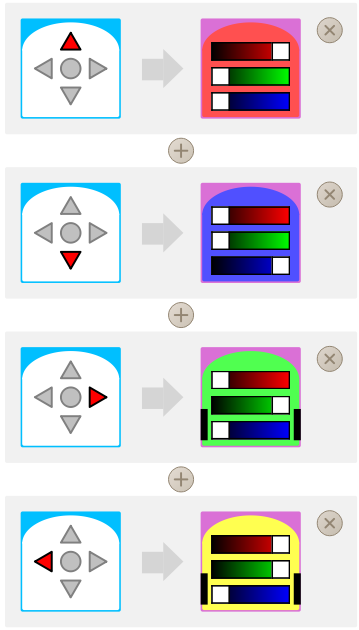
\includegraphics[width = 0.4\textwidth]{colors1}
	}
    \hspace{1.5cm}
    \subfigure[Éteindre Thymio lorsque le bouton centrale est touché]{
		\label{fig.colors-b}
		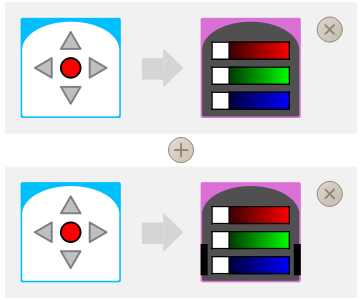
\includegraphics[width = 0.4\textwidth]{colors2}
	}
    \caption{Jouer avec les lumières de Thymio}
    \label{fig.colors}
\end{figure}
